Карта глубины — это изображение, на котором для каждого пикселя, вместо цвета, храниться его расстояние до камеры. Карта глубины может быть построена по стереопаре изображений.

Идея, лежащая в основе построения карты глубины по стереопаре следующая: для каждой точки на одном изображении выполняется поиск парной ей точки на другом изображении. По паре соответствующих точек можно выполнить триангуляцию и определить координаты их прообраза в трехмерном пространстве. Зная трехмерные координаты прообраза, глубина вычисляется, как расстояние до плоскости камеры.

Парную точку нужно искать на эпиполярной линии. Для упрощения поиска, изображения выравнивают так, что бы все эпиполярные линии были параллельны сторонам изображения (обычно горизонтальны). Изображения выравнивают так, что бы для точки с координатами $(x_0, y_0)$ соответствующая ей эпиполярная линия задавалась уравнением $x = x_0$, тогда для каждой точки соответствующую ей парную точку нужно искать в той-же строчке на изображении со второй камеры. Такой процесс выравнивания изображений называют ректификацией. Обычно ректификацию совершают путем ремаппинга изображения и ее совмещают с избавлением от дисторсий.

После того как изображения ректифицированы, выполняют поиск соответствующих пар точек. Самый простой способ проиллюстрирован на рисунке \ref{img:approach} и состоит в следующем: для каждого пикселя левой картинки с координатами $(x_0, y_0)$ выполняется поиск пикселя на правой картинке. При этом предполагается, что пиксель на правой картинке должен иметь координаты $(x_0 - d, y_0)$, где $d$ — величина называемая несоответствием или смещением (disparity). Поиск соответствующего пикселя выполняется путем вычисления максимума функции отклика, в качестве которой может выступать, например, корреляция окрестностей пикселей.

\begin{figure}[!h]
	\center {
		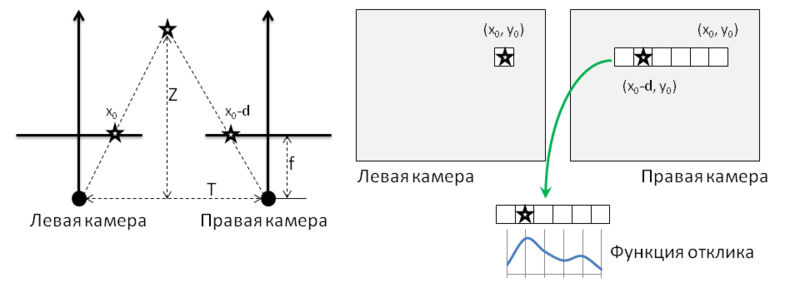
\includegraphics[width=\linewidth]{img/approach}
	}
	\caption{Метод поиска соответствующих пар проекций точек на стереопару.}
	\label{img:approach}
\end{figure}